\documentclass{ximera}

\title{CH 3 Intro to Functions Exercises}

\begin{document}

In Exercises 1 - 2, use the given function $f$ to find $f(0)$ and solve $f(x) = 0$ 

\begin{exercise}
$f(x) = 2x - 1$

\begin{prompt}
$f(0)=\answer{-1}$ $x=\answer{\frac{1}{2}}$
\end{prompt}
\end{exercise}
\begin{exercise}
 $f(x) = 3 - \frac{2}{5} x$
 
 \begin{prompt}
 $f(0)=\answer{3}$ $x=\answer{\frac{15}{2}}$
 \end{prompt}

\end{exercise}
\begin{exercise}
\[
 \graph[]{}
\]
\end{exercise}
\begin{image}
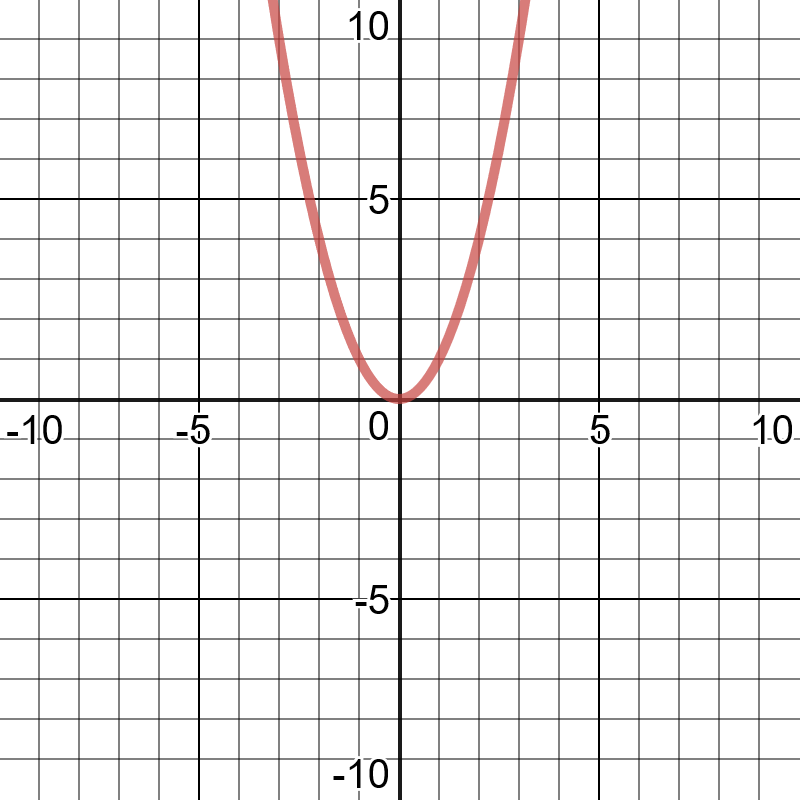
\includegraphics[]{desmos-graph.png}    
\end{image}



\end{document}
